\documentclass[dvipsnames]{beamer}
\usepackage{lmodern}
\usepackage{appendixnumberbeamer}
\renewcommand{\sfdefault}{lmss}
\renewcommand{\ttdefault}{lmtt}
\usepackage[T1]{fontenc}
% \usepackage[utf8]{inputenc}
\setcounter{secnumdepth}{3}
\setcounter{tocdepth}{3}
\usepackage{amsmath}
\usepackage{amsthm}
\usepackage{amssymb}
\theoremstyle{definition}
\newtheorem*{defn*}{\protect\definitionname}
\providecommand{\definitionname}{Definition}
\usepackage{graphicx}
\usepackage{hyperref}
\usepackage{ulem}
\PassOptionsToPackage{normalem}{ulem}
\usepackage{caption}
\usepackage{subcaption}
\usepackage{verbatim}
\usepackage[english]{babel}
\usepackage[autostyle]{csquotes}
\usepackage{tikz}
\usetikzlibrary{arrows,intersections}
\usepackage{pgfplots}
\pgfplotsset{compat = 1.15}
\usepgfplotslibrary{fillbetween}
\usepackage{verbatim}
\usepackage{booktabs}
\usepackage{multirow}
\usepackage{array}
\usepackage{nccmath}
% \usepackage{listings}
\usepackage{mathtools}

%Bibliography style, etc.
\usepackage[citestyle=authoryear-comp,natbib, uniquename = false, url = false, doi = false, uniquelist=false]{biblatex}
\renewbibmacro{in:}{}
\AtEveryBibitem{%
  \clearfield{volume}%
  \clearfield{number}
  \clearfield{month}
  \clearfield{issn}
  \clearfield{isbn}
  \clearfield{pages}
}

%\usepackage{cleveref}
\usepackage{setspace}
\makeatletter

% Macros
\providecommand{\tabularnewline}{\\}
\newcommand{\gr}{\textcolor{ForestGreen}} 
\newcommand{\rd}{\textcolor{red}}
\newcommand{\cb}{\textcolor{CornflowerBlue}} %this is the blue color you like; simply type \cb{X} where "X" is the color you want in blue
\newcommand{\vitem}{\vfill \item} %auto-centers items in lists
\newcommand{\fall}{\ \forall} %redefines "forall" (I don't like the default spacing)
\newcommand{\frall}{\quad \forall} %a \forall separated from the main math; this is the way it usually shows up in equations
\newcommand{\exist}{\ \exists} %same as \fall, but for \exists; they have the same ugly spacing
\newcommand{\R}{\mathbb{R}} %set of real numbers
\newcommand*\bigcdot{\mathpalette\bigcdot@{.5}} %different size for cdots
% \newcommand{\argmax}{\text{arg}\max}
\newenvironment{itemframe}
    {\frame{}\itemize}
    {\itemize\frame}
\newcommand\makebeamertitle{\frame{\maketitle}}%
\newtheoremstyle{named}{}{}{\itshape}{}{\bfseries}{.}{.5em}{\thmnote{#3's }#1}
\theoremstyle{named}
\newtheorem*{prop*}{Proposition}
% \newtheorem*{corollary}{Corollary}
\newtheorem*{namedtheorem}{Theorem} %allows named theorems
\newtheorem*{nameddef}{Definition}
\newtheorem{proposition}{Proposition}
\newtheorem*{assumption}{Assumption}
\newtheorem*{namedcorollary}{Corollary}
\newtheorem*{namedlemma}{Lemma}
\newtheorem*{axiom}{Axiom}
\newtheorem*{theorem*}{Theorem}
\newtheorem*{lemma*}{Lemma}
\DeclareMathOperator*{\argmin}{argmin}
\DeclareMathOperator{\argmax}{argmax}
\DeclareMathOperator{\supp}{supp}
\DeclareMathOperator{\interior}{int}
\DeclareMathOperator{\rank}{rank}
\newcolumntype{C}[1]{>{\centering\let\newline\\\arraybackslash\hspace{0pt}}m{#1}}
\newcommand{\sbt}{\,\begin{picture}(-1,1)(-1,-3)\circle*{2}\end{picture}\ }



%formatting
\usetheme{Ilmenau}
\definecolor{MIT}{rgb}{.639,.122,.204}
\definecolor{UCLA}{rgb}{0.15294117647058825, 0.4549019607843137, 0.6823529411764706}
\definecolor{UCLA_gold}{rgb}{1, 0.8196078431372549, 0}
\usecolortheme[named=UCLA]{structure}
\setbeamercolor*{palette secondary}{fg=UCLA_gold,bg=gray!15!white}
\usecolortheme{dolphin}
\setbeamertemplate{navigation symbols}{} 
\setbeamertemplate{footline}{}{}
\setbeamertemplate{headline}{}
\setbeamertemplate{navigation symbols}{}
\mode<presentation> {}
\setbeamercolor{block title}{use=structure,fg=white,bg=RoyalBlue} %blocks (theorems, etc.)in blue
\setbeamercolor{block title alerted}{use=structure,fg=white,bg=ForestGreen} %blocks (theorems, etc.)in blue

\renewcommand\qedsymbol{$\blacksquare$} %set QED symbol as black square
\renewcommand{\emph}{\textit} %set emphasized text style; this is italics
\setbeamertemplate{footline}[frame number] %slide numbers
\setbeamertemplate{itemize item}[circle] %bullet style
\setbeamertemplate{itemize subitem}{--}
\setbeamertemplate{enumerate item}[default]
\newrobustcmd*{\parentexttrack}[1]{%
  \begingroup
  \blx@blxinit
  \blx@setsfcodes
  \blx@bibopenparen#1\blx@bibcloseparen
  \endgroup}

\AtEveryCite{%
  \let\parentext=\parentexttrack%
  \let\bibopenparen=\bibopenbracket%
  \let\bibcloseparen=\bibclosebracket}

 \AtBeginDocument{%
   \let\origtableofcontents=\tableofcontents
   \def\tableofcontents{\@ifnextchar[{\origtableofcontents}{\gobbletableofcontents}}
   \def\gobbletableofcontents#1{\origtableofcontents}
 }
\newcommand{\backupbegin}{
   \newcounter{framenumberappendix}
   \setcounter{framenumberappendix}{\value{framenumber}}
}
\newcommand{\backupend}{
   \addtocounter{framenumberappendix}{-\value{framenumber}}
   \addtocounter{framenumber}{\value{framenumberappendix}} 
} 

\renewcommand{\maketitle}{
\setbeamertemplate{footline}{} 
\begin{frame}[noframenumbering]
\titlepage
\end{frame}
\setbeamertemplate{footline}[frame number]
}

\usefonttheme[onlymath]{serif}

% \usetheme{CambridgeUS}

% \newtheorem{theorem}{Theorem}
% \theoremstyle{claim}
\newtheorem{claim}{Claim}
% \newtheorem{corollary}{Corollary}


\makeatother


%\author{Drew Fudenberg}

\institute[]{}
\title{Detection of Bid Rigging in Procurement Auctions}
\author{Porter and Zona (\emph{JPE} 1993)}
\date{\today}

\begin{document}
\maketitle
\begin{frame}{Overview}
  \begin{itemize}
  \item Authors suspect construction firms of engaging in bid-rigging
    \vitem They want to test whether the observed bidding behavior can be explained by competitive behavior
    \vitem Split the firms into two groups (cartel firms and competitive firms) and see if their behavior is the same
  \end{itemize}
\end{frame}
%
\begin{frame}{How these bids work}
  \begin{enumerate}
  \item Interested firms request plans and specifications (the list of interested firms is public info)
    \vitem On the ``auction day'', each bidder's sealed bid is opened and announced to everyone present
    \vitem The lowest bid is accepted, provided it is ``responsible'' (direct quote)
    \vitem If the DOT determines that the bid is responsible, they accept it and publicize the bids and awarded contracts
  \end{enumerate}
\end{frame}
%
\begin{frame}{Why do we expect collusion?}
  \begin{itemize}
  \item One of the firms already got caught rigging bids
    \vitem Firms \emph{only} compete on prize (no differentiated goods)
    \vitem Public DOT announcements allow for detection of and punishment for non-cooperative behavior
    \vitem Buyer lists ensure common knowledge prior to the auction
    \vitem Largely inelastic demand (bidders keep any increase in price)
  \end{itemize}
\end{frame}
%
\begin{frame}{Model/Bid Levels}
  \begin{itemize}
  \item IPV Auction
    \begin{equation}
\varphi_{it} (b_{it}) + (b_{it} - c_{it})\frac{\partial \varphi_{it}(b_{it})}{\partial b} = 0\tag{FOC}
    \end{equation}
    \vitem Assume equilibrium behavior satisfies log-linear bidding rule (\rd{restrictive assumption}):
    \[
\log (b_{it}) = \alpha_t + \beta \mathbf{X}_{it} + \varepsilon_{it}
    \]
    \vitem Emphasizes between-firm instead of between-job differences
    \begin{itemize}
    \item This part of the data is more informative
    \end{itemize}
    \vitem Estimate this via OLS; compare the coefficients for cartel members and other firms
  \end{itemize}
\end{frame}
%
\begin{frame}{Bid Ranking}
  \begin{itemize}
  \item Competitive firms need to balance their expected profits against their probability of winning
    \vitem Cartel firms \emph{know} that their probability of winning is $0$ if they aren't the designated low-bidder
    \vitem The (approximate) probability of submitting the lowest bid is
    \[
\ln P[b_{it} < b_{jt}, \forall j \ne i] = \theta_t + \beta \frac{\mathbf{X}_{it}}{\sigma_t} \sqrt{\frac{\pi}{6}} \tag{MNL }
    \]
    \vitem Estimate the standard deviations for each auction, then
    \begin{align*}
      \ln P [b_{it} < b_{jt}, \forall j \ne i] &= \alpha_t + \beta Z_{it}\\
      \implies P [b_{it} < b_{jt}, \forall j \ne i] &= \frac{e^{\beta Z_{it}}}{\sum_je^{\beta Z_{jt}}}
                                           \end{align*}
  \end{itemize}
\end{frame}
%
\begin{frame}{Bid Ranking}
  \begin{itemize}
  \item We can combine all these probability to get the probability of seeing a specific bid ranking \gr{in a given auction},
    \[
P[b_{r1t} < b_{r2t} < \ldots < b_{rnt}] = \prod^{n_t}_{i = 1} \frac{e^{\beta Z_{r_i}t}}{\sum^{n_t}_{j = i} e^{\beta Z r_j t}}
    \]
    \vitem And now combine all these guys to get the probability of seeing the actual rankings in the data \rd{across all auctions},
    \[
L(\beta) = \prod^T_{t = 1} \prod^{n_t}_{i = 1} \frac{e^{\beta Z_{r_i}t}}{\sum^{n_t}_{j = i} e^{\beta Z r_j t}}
    \]
  \end{itemize}
\end{frame}
%
\begin{frame}{MLE Estimation and Hypothesis Testing}
  \begin{itemize}
  \item If the model is correctly specified, we can use any subset of the data to estimate the parameters.
    \vitem Split the data into cartel firms and competitive firms.
    \vitem Hausman test that the parameters are the same.
    \vitem If they're not the same, then we have suggestive evidence of ``phantom bidding'' or other weird behavior by the cartel firms.
  \end{itemize}
\end{frame}
%
\begin{frame}{Are Competitive and Cartel Firms the Same? Levels}
  \begin{center}
   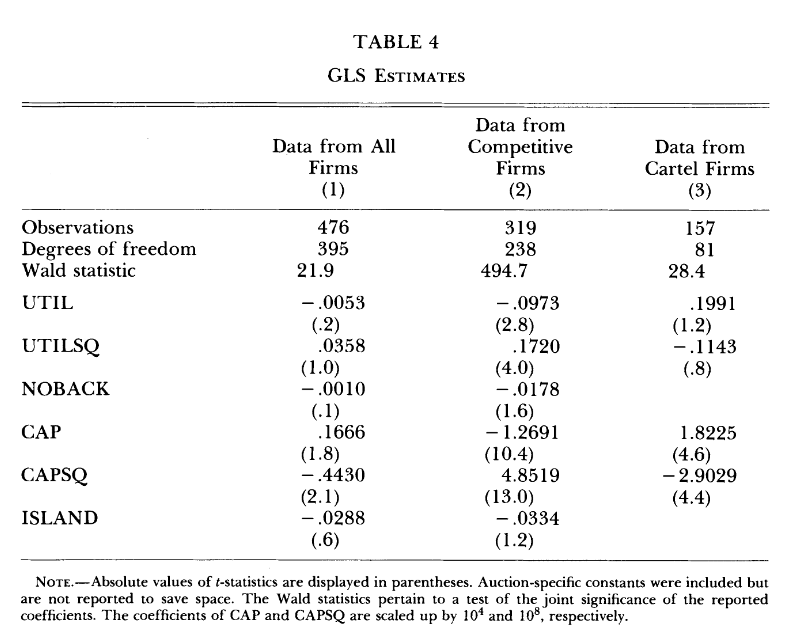
\includegraphics[width=0.75\textwidth, keepaspectratio=true]{tab4.png}
  \end{center}
  \begin{itemize}
  \item The model fits the competitive data pretty well
    \vitem Bids from cartel firms are statistically different from competitive firms' bids
  \end{itemize}
\end{frame}
%
\begin{frame}{Competitive Rank Based Estimates}
  \begin{center}
   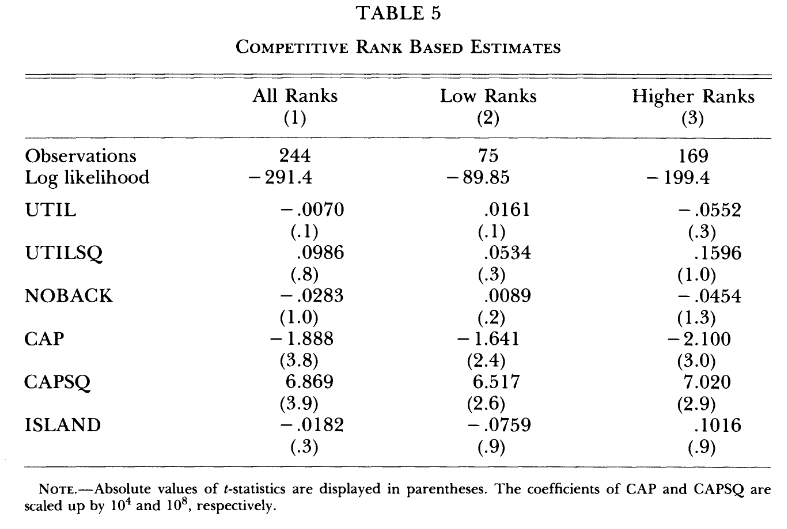
\includegraphics[width=\textwidth, keepaspectratio=true]{tab5.png} 
  \end{center}
  \begin{itemize}
  \item \gr{Cannot} reject the null that low bids and non-low bids are generated by the same DGP.
  \end{itemize}
\end{frame}
%
\begin{frame}{Cartel Rank Based Estimates}
  \begin{center}
   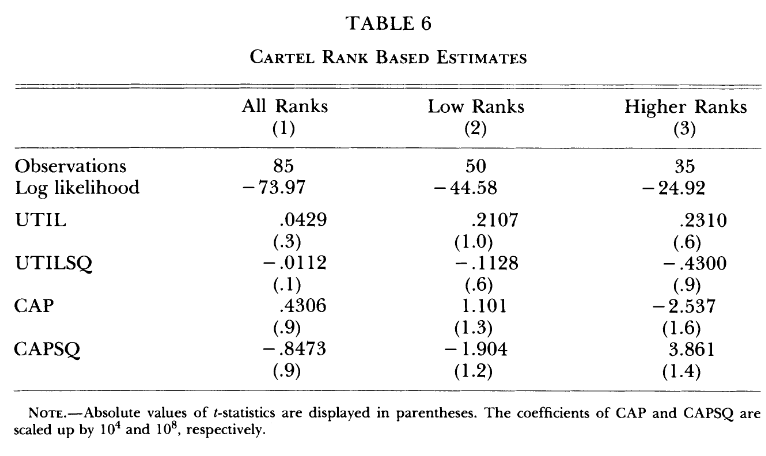
\includegraphics[width=\textwidth, keepaspectratio=true]{tab6.png}
  \end{center}
  \begin{itemize}
  \item \rd{Reject} the null of no phantom bidding
    \vitem Conclude that cartel bids \gr{are} generated by a different process depending on whether they are low or not
  \end{itemize}
\end{frame}
%
\begin{frame}{Wrapping Up}
  \begin{itemize}
  \item Features in the DOT auction market make it susceptible to bid rigging
    \vitem There is a group of candidate cartel firms, and a group of non-cartel firms
    \vitem The authors estimate the firms' parameters and impose some restrictions on the bidding functions they can be using.
    \vitem Non-cartel firms behave the same whether they win or lose; they're trying to maximize their expected profits as a function of surplus and probability of winning.
    \vitem Cartel firms do something different; they aren't trying to maximize profits when they submit non-winning bids, since they know another cartel member will win anyway.
  \end{itemize}
\end{frame}
\end{document}
%%% Local Variables:
%%% mode: latex
%%% TeX-master: t
%%% End:
